\documentclass[11pt]{article}

% This first part of the file is called the PREAMBLE. It includes
% customizations and command definitions. The preamble is everything
% between \documentclass and \begin{document}.

\usepackage[margin=1in]{geometry}  % set the margins to 1in on all sides

\usepackage{graphicx}              % to include figures
\usepackage{amsmath}               % great math stuff
\usepackage{amsfonts}              % for blackboard bold, etc
\usepackage{amsthm}                % better theorem environments

\usepackage{dcolumn}
\usepackage{dsfont}
\usepackage{array}
\usepackage{booktabs}
\usepackage{soul}
\usepackage{mathrsfs}
\usepackage{enumerate}
\usepackage{multicol}
\usepackage[makeroom]{cancel}
\usepackage{xcolor}
\usepackage{tikz}
\usepackage{pdfpages}

% various theorems, numbered by section

\newtheorem{thm}{Theorem}[section]
\newtheorem{lem}[thm]{Lemma}
\newtheorem{prop}[thm]{Proposition}
\newtheorem{cor}[thm]{Corollary}
\newtheorem{conj}[thm]{Conjecture}
\newtheorem{exer}[thm]{Exercise}

\DeclareMathOperator{\id}{id}

\newcommand{\EE}{\mathbb{E}}
\newcommand{\ff}{\boldsymbol{f}}
\newcommand{\Hl}{\boldsymbol{H}_\lambda}
\newcommand{\II}{\boldsymbol{I}}
\newcommand{\ee}{\boldsymbol{e}}
\newcommand{\yy}{\boldsymbol{y}}
\newcommand{\bd}[1]{\mathbf{#1}}  % for bolding symbols
\newcommand{\RR}{\mathbb{R}}      % for Real numbers
\newcommand{\ZZ}{\mathbb{Z}}      % for Integers
\newcommand{\col}[1]{\left[\begin{matrix} #1 \end{matrix} \right]}
\newcommand{\comb}[2]{\binom{#1^2 + #2^2}{#1+#2}}
\newcommand{\overfrac}[2]{\genfrac{}{}{0pt}{}{#1}{#2}}

\renewcommand{\thesubsection}{\thesection.\alph{subsection}}

\everymath{\displaystyle}

\setlength\parindent{0pt}

\usepackage{setspace}

\begin{document}
\begin{multicols}{2}
  \phantom{hello}\vspace{0.01\baselineskip}
  \phantom{hello}\vspace{0.01\baselineskip}
  {\large Assignment 4}\\
  \begin{flushright}
    Mikhail Gaerlan (914437675)\\
    21 April 2017\\
    STA 243 Lee
  \end{flushright}
\end{multicols}
\vspace{-2.3\baselineskip}

\hrulefill

\section{}

The black line represents the true function, the blue line represents the unpenalized regression spline, and the red line represents the penalized regression spline. The \texttt{nlm} command in R was used to minimize the following expressions.

\subsection{}

\subsubsection{Cross Validation}

\subsubsection{Generalized Cross Validation}

\subsection{Corrected Akaike Information Criterion}

\subsection{Risk Minimization}

\begin{eqnarray*}
  \EE\lVert\yy-\hat{\mathbf{f}}_\lambda\rVert^2&=&\EE\lVert\yy-\Hl\yy\rVert^2\\
                                               &=&\EE\lVert\left(\II-\Hl\right)\yy\rVert^2\\
                                               &=&\EE\lVert\left(\II-\Hl\right)\left(\ff+\ee\right)\rVert^2\\
                                               &=&\EE\lVert\left(\II-\Hl\right)\ff+\left(\II-\Hl\right)\ee\rVert^2\\
                                               &=&\EE\lVert\left(\II-\Hl\right)\ff\rVert^2+\EE\lvert\left(\II-\Hl\right)\ee\rVert^2+2\EE\left[\left(\II-\Hl\right)\ff\cdot\left(\II-\Hl\right)\ee\right]\\
                                               &=&\lVert\left(\II-\Hl\right)\ff\rVert^2+\EE\left[\left(\ff-\Hl\ff\right)\cdot\left(\ee-\Hl\ee\right)\right]\\
                                               &=&\lVert\left(\II-\Hl\right)\ff\rVert^2+\EE\left[\ff\cdot\left(\ee-\Hl\ee\right)-\Hl\ff\cdot\left(\ee-\Hl\ee\right)\right]\\
                                               &=&\lVert\left(\II-\Hl\right)\ff\rVert^2+\EE\left[\ff\cdot\ee-\ff\cdot\Hl\ee-\Hl\ff\cdot\ee+\Hl\ff\cdot\Hl\ee\right]\\
                                               &=&\lVert\left(\II-\Hl\right)\ff\rVert^2+\EE\left[\ff\cdot\ee-\Hl^T\ff\cdot\ee-\Hl\ff\cdot\ee+\Hl^T\Hl\ff\cdot\ee\right]\\
                                               &=&\lVert\left(\II-\Hl\right)\ff\rVert^2+\EE\left[\left(\II-\Hl^T-\Hl+\Hl^T\Hl\right)\ff\cdot\ee\right]\\
                                               &=&\lVert\left(\II-\Hl\right)\ff\rVert^2+\textrm{Cov}\left(\ee\right)\left(\II-\Hl-\Hl^T-\Hl^T\Hl\right)\\
                                               &=&\lVert\left(\II-\Hl\right)\ff\rVert^2+\sigma^2\left\{\textrm{tr}\left(\Hl\Hl^T\right)-2\textrm{tr}\left(\Hl\right)+n\right\}
\end{eqnarray*}

\begin{table*}[h]
  \begin{center}
    \renewcommand{\arraystretch}{1.5}
    \begin{tabular}{| >{\centering\arraybackslash}m{2.1in} |  >{\centering\arraybackslash}m{2.1in} |  >{\centering\arraybackslash}m{2.1in}|}
      \hline
      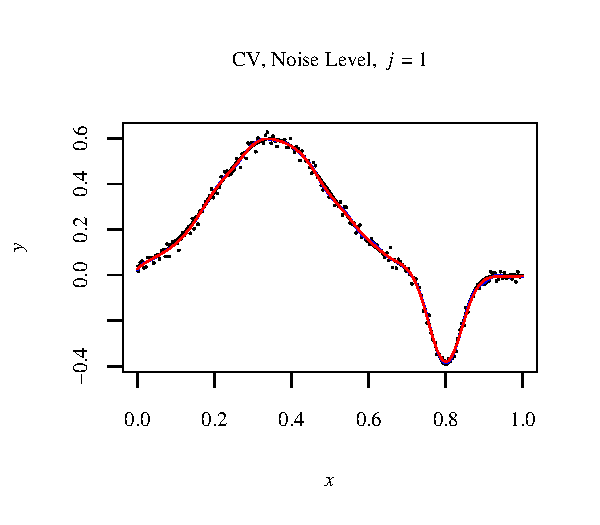
\includegraphics[width=1\linewidth,height=0.18\textheight]{Graphs/1/1/assignment5_a_1_1_1}&
      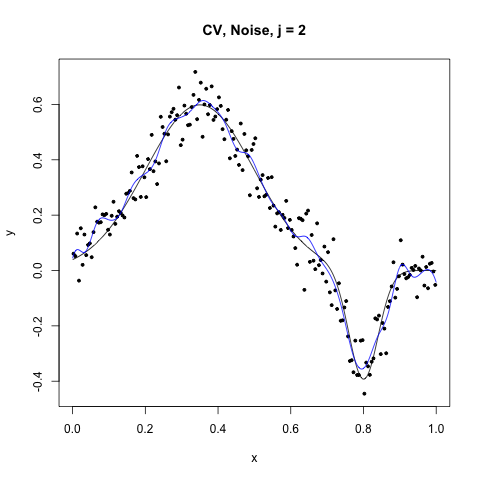
\includegraphics[width=1\linewidth,height=0.18\textheight]{Graphs/1/1/assignment5_a_1_1_2}&
      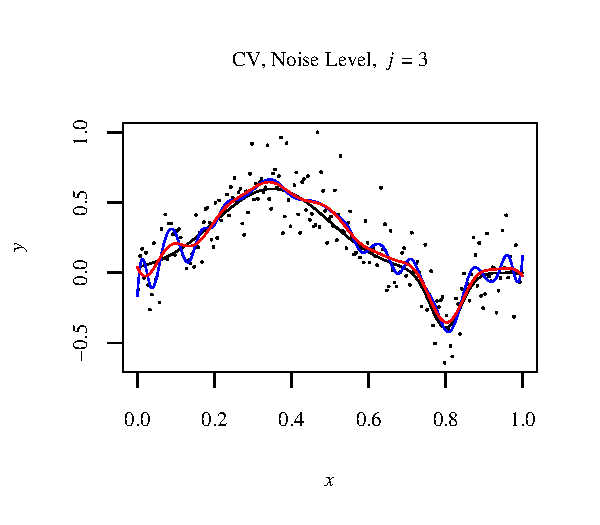
\includegraphics[width=1\linewidth,height=0.18\textheight]{Graphs/1/1/assignment5_a_1_1_3}\\\hline
      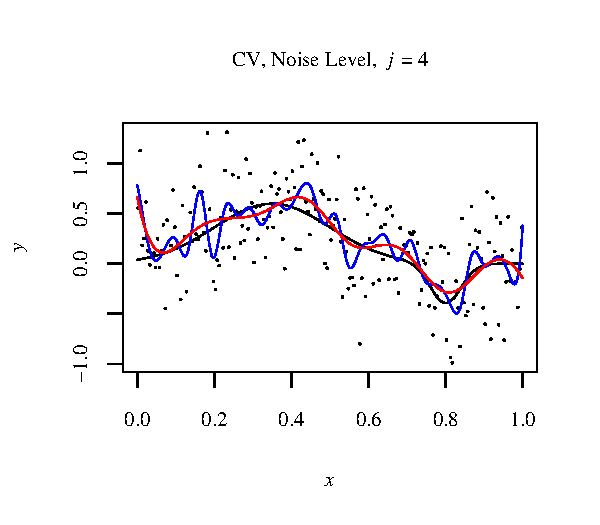
\includegraphics[width=1\linewidth,height=0.18\textheight]{Graphs/1/1/assignment5_a_1_1_4}&
      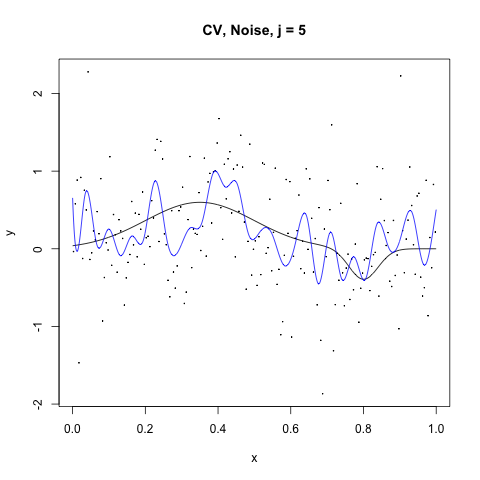
\includegraphics[width=1\linewidth,height=0.18\textheight]{Graphs/1/1/assignment5_a_1_1_5}&
      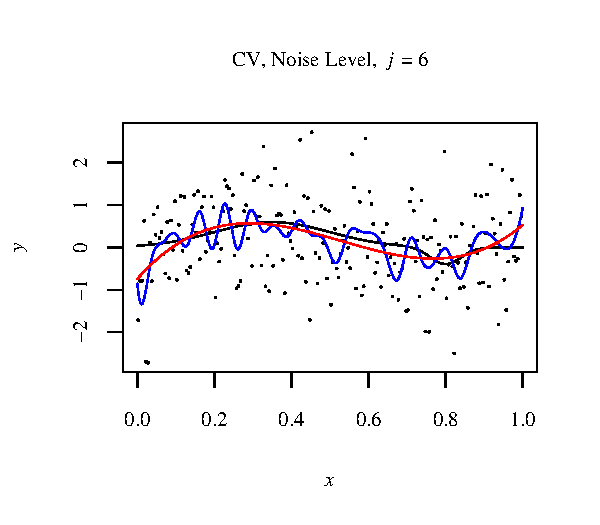
\includegraphics[width=1\linewidth,height=0.18\textheight]{Graphs/1/1/assignment5_a_1_1_6}\\\hline
    \end{tabular}
  \end{center}
\end{table*}

\begin{table*}[h!]
  \begin{center}
    \renewcommand{\arraystretch}{1.5}
    \begin{tabular}{| >{\centering\arraybackslash}m{2.1in} |  >{\centering\arraybackslash}m{2.1in} |  >{\centering\arraybackslash}m{2.1in}|}
      \hline
      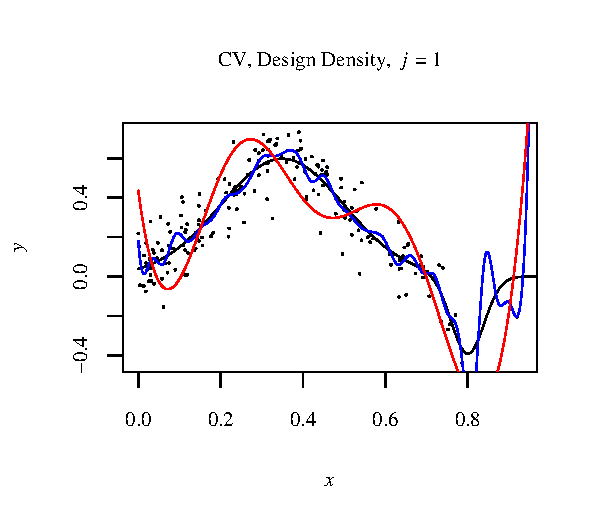
\includegraphics[width=1\linewidth,height=0.18\textheight]{Graphs/1/2/assignment5_a_1_2_1}&
      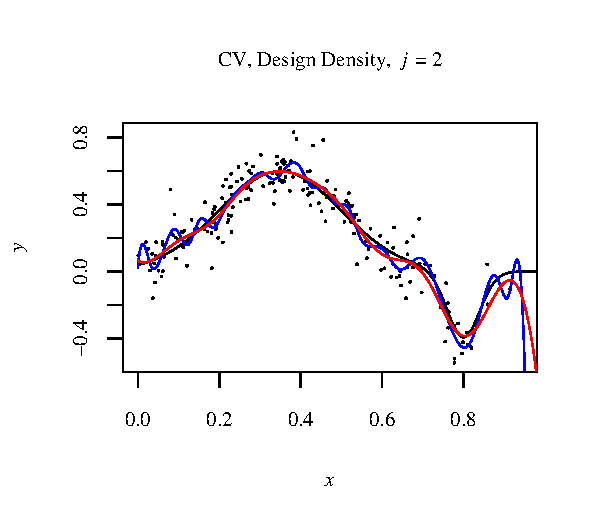
\includegraphics[width=1\linewidth,height=0.18\textheight]{Graphs/1/2/assignment5_a_1_2_2}&
      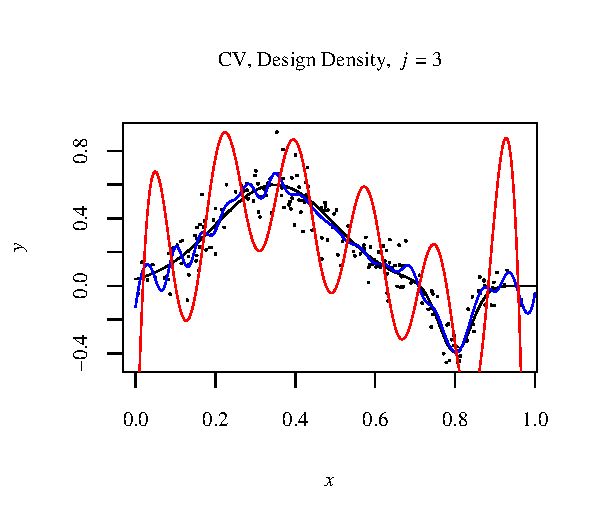
\includegraphics[width=1\linewidth,height=0.18\textheight]{Graphs/1/2/assignment5_a_1_2_3}\\\hline
      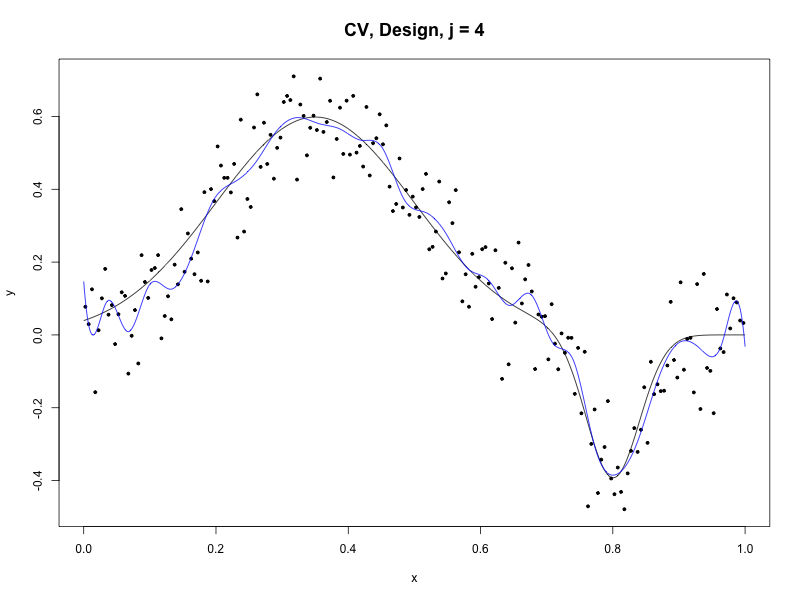
\includegraphics[width=1\linewidth,height=0.18\textheight]{Graphs/1/2/assignment5_a_1_2_4}&
      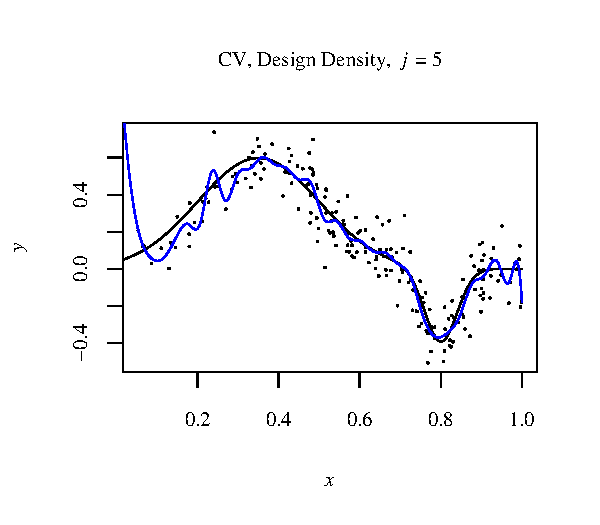
\includegraphics[width=1\linewidth,height=0.18\textheight]{Graphs/1/2/assignment5_a_1_2_5}&
      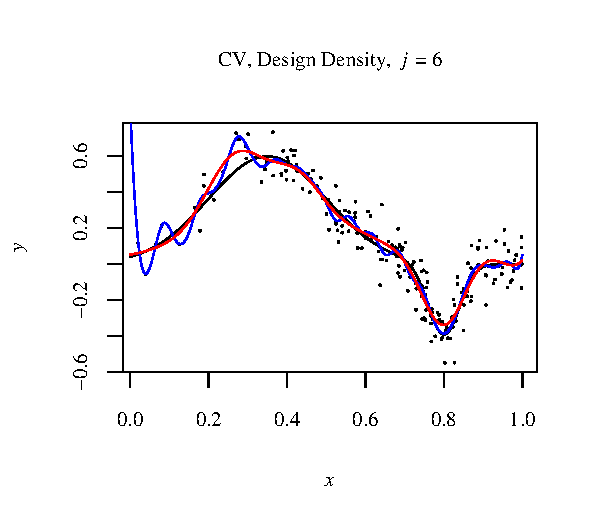
\includegraphics[width=1\linewidth,height=0.18\textheight]{Graphs/1/2/assignment5_a_1_2_6}\\\hline
    \end{tabular}
  \end{center}
\end{table*}

\begin{table*}[h!]
  \begin{center}
    \renewcommand{\arraystretch}{1.5}
    \begin{tabular}{| >{\centering\arraybackslash}m{2.1in} |  >{\centering\arraybackslash}m{2.1in} |  >{\centering\arraybackslash}m{2.1in}|}
      \hline
      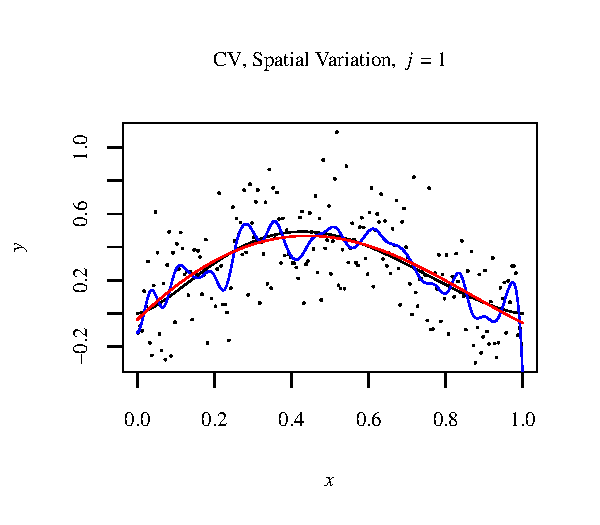
\includegraphics[width=1\linewidth,height=0.18\textheight]{Graphs/1/3/assignment5_a_1_3_1}&
      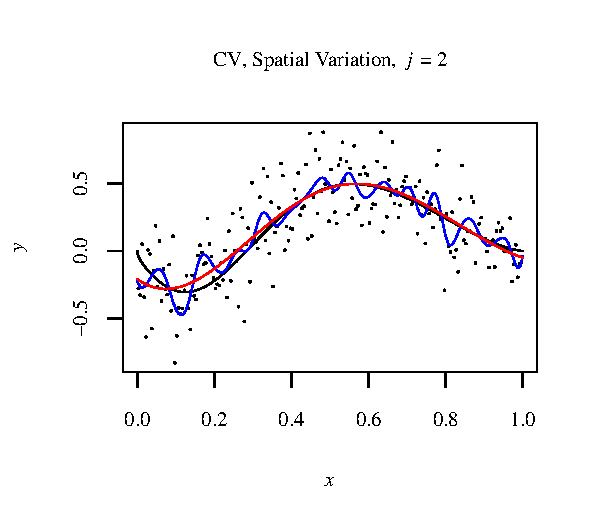
\includegraphics[width=1\linewidth,height=0.18\textheight]{Graphs/1/3/assignment5_a_1_3_2}&
      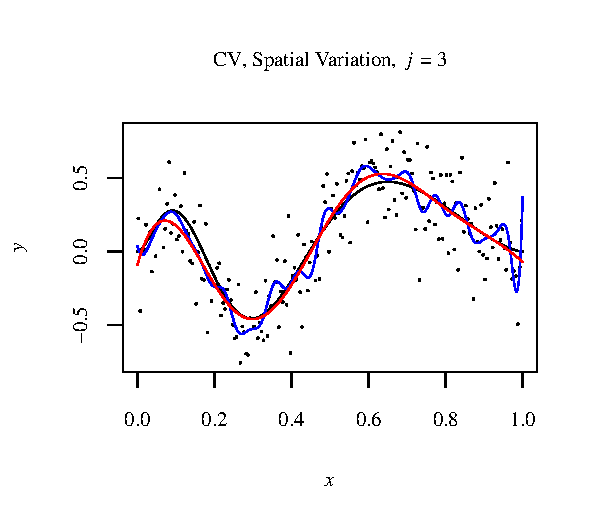
\includegraphics[width=1\linewidth,height=0.18\textheight]{Graphs/1/3/assignment5_a_1_3_3}\\\hline
      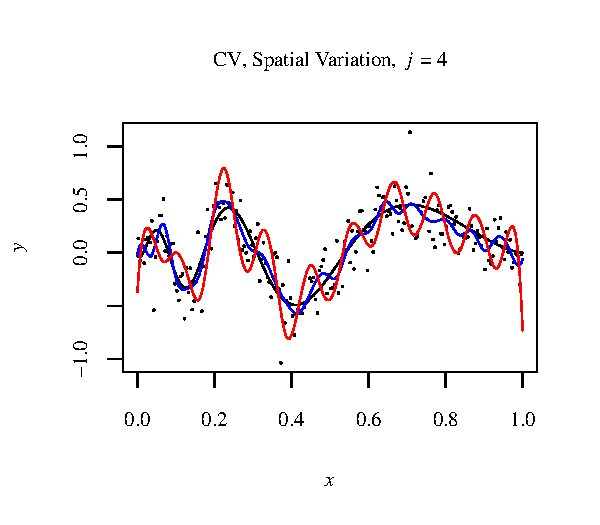
\includegraphics[width=1\linewidth,height=0.18\textheight]{Graphs/1/3/assignment5_a_1_3_4}&
      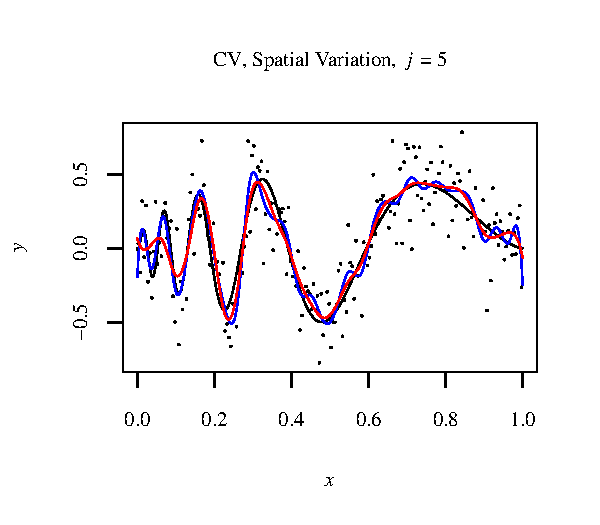
\includegraphics[width=1\linewidth,height=0.18\textheight]{Graphs/1/3/assignment5_a_1_3_5}&
      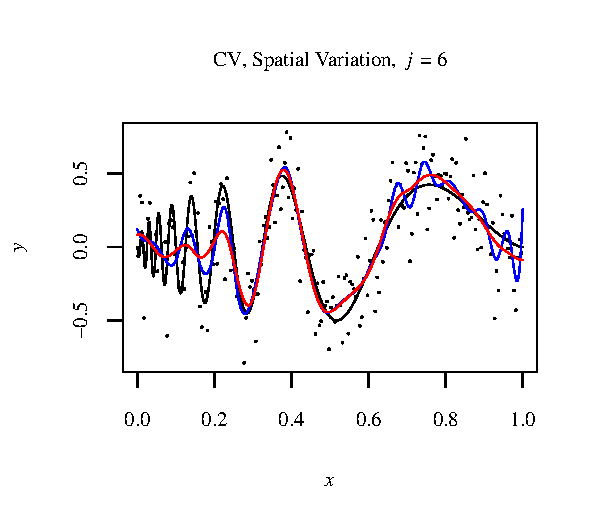
\includegraphics[width=1\linewidth,height=0.18\textheight]{Graphs/1/3/assignment5_a_1_3_6}\\\hline
    \end{tabular}
  \end{center}
\end{table*}

\begin{table*}[h!]
  \begin{center}
    \renewcommand{\arraystretch}{1.5}
    \begin{tabular}{| >{\centering\arraybackslash}m{2.1in} |  >{\centering\arraybackslash}m{2.1in} |  >{\centering\arraybackslash}m{2.1in}|}
      \hline
      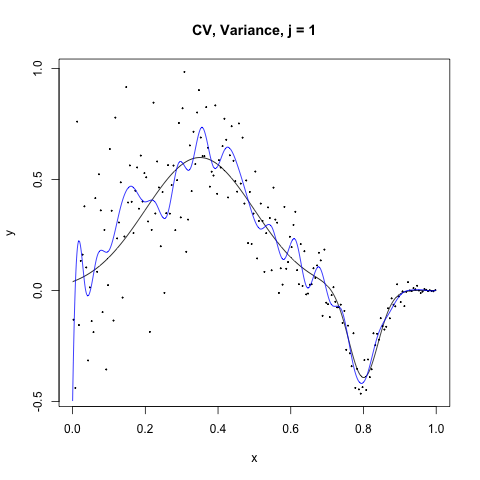
\includegraphics[width=1\linewidth,height=0.18\textheight]{Graphs/1/4/assignment5_a_1_4_1}&
      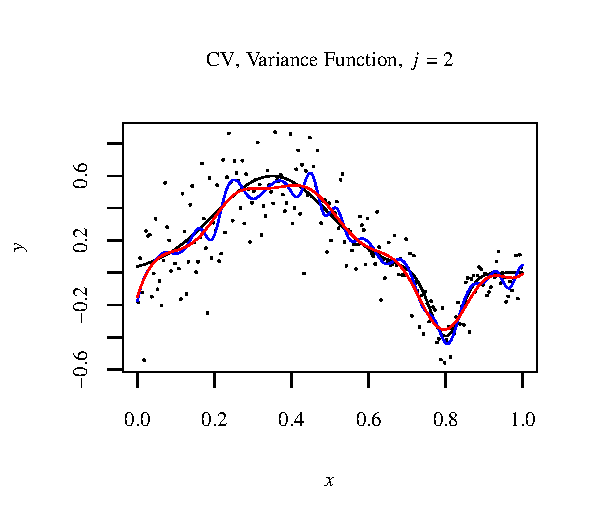
\includegraphics[width=1\linewidth,height=0.18\textheight]{Graphs/1/4/assignment5_a_1_4_2}&
      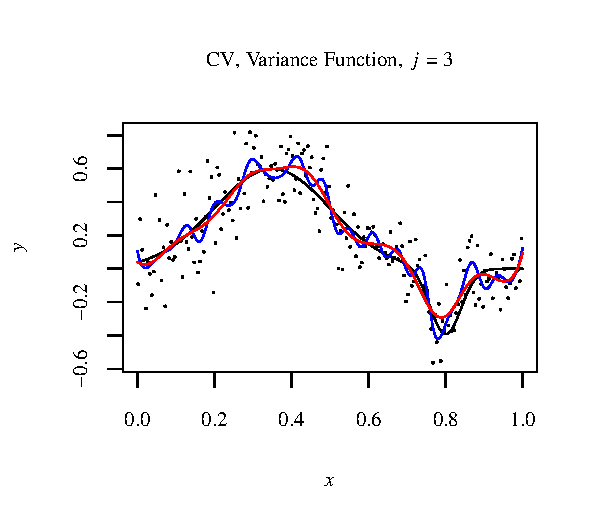
\includegraphics[width=1\linewidth,height=0.18\textheight]{Graphs/1/4/assignment5_a_1_4_3}\\\hline
      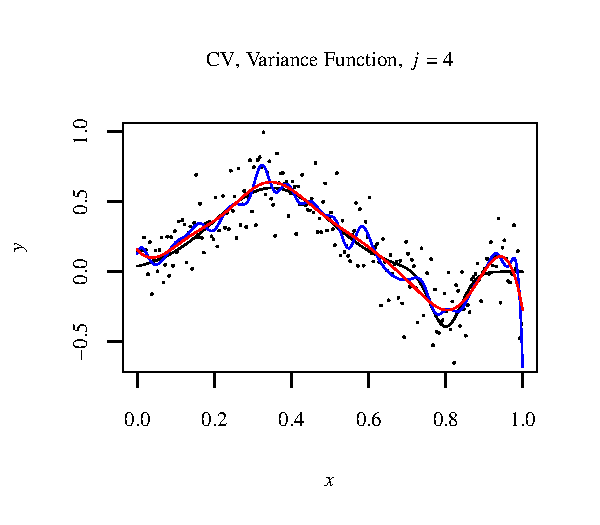
\includegraphics[width=1\linewidth,height=0.18\textheight]{Graphs/1/4/assignment5_a_1_4_4}&
      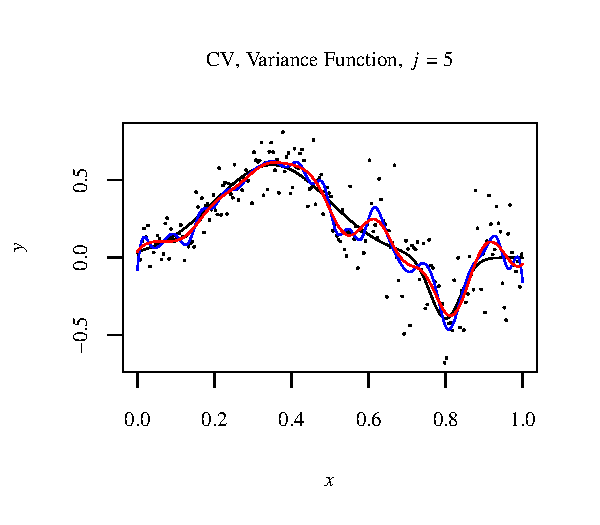
\includegraphics[width=1\linewidth,height=0.18\textheight]{Graphs/1/4/assignment5_a_1_4_5}&
      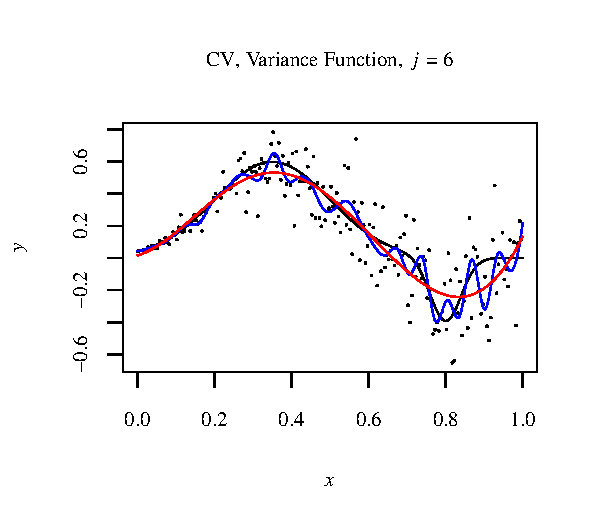
\includegraphics[width=1\linewidth,height=0.18\textheight]{Graphs/1/4/assignment5_a_1_4_6}\\\hline
    \end{tabular}
  \end{center}
\end{table*}

\begin{table*}[h!]
  \begin{center}
    \renewcommand{\arraystretch}{1.5}
    \begin{tabular}{| >{\centering\arraybackslash}m{2.1in} |  >{\centering\arraybackslash}m{2.1in} |  >{\centering\arraybackslash}m{2.1in}|}
      \hline
      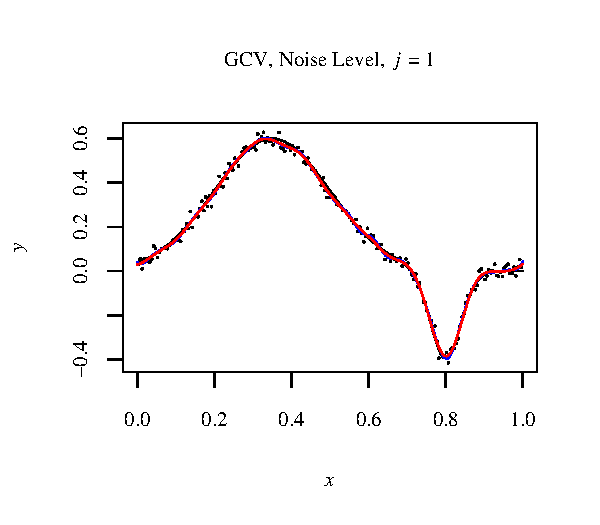
\includegraphics[width=1\linewidth,height=0.18\textheight]{Graphs/2/1/assignment5_a_2_1_1}&
      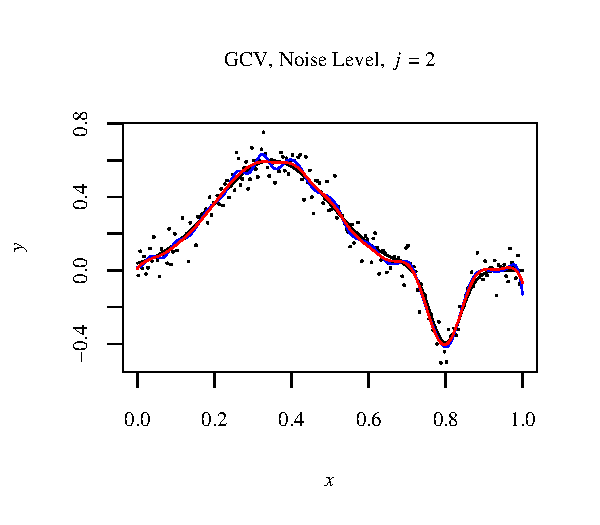
\includegraphics[width=1\linewidth,height=0.18\textheight]{Graphs/2/1/assignment5_a_2_1_2}&
      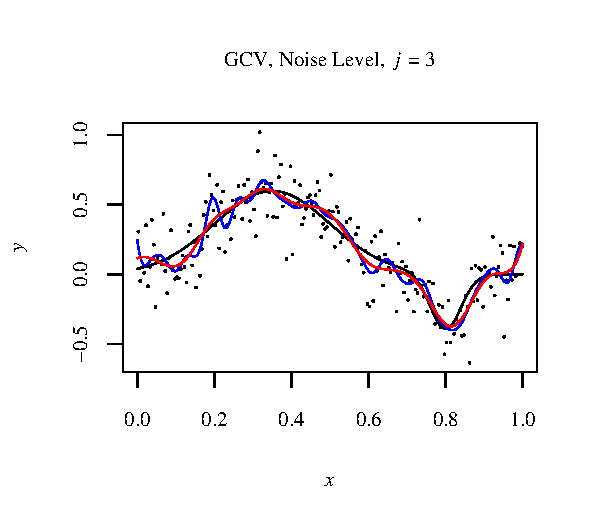
\includegraphics[width=1\linewidth,height=0.18\textheight]{Graphs/2/1/assignment5_a_2_1_3}\\\hline
      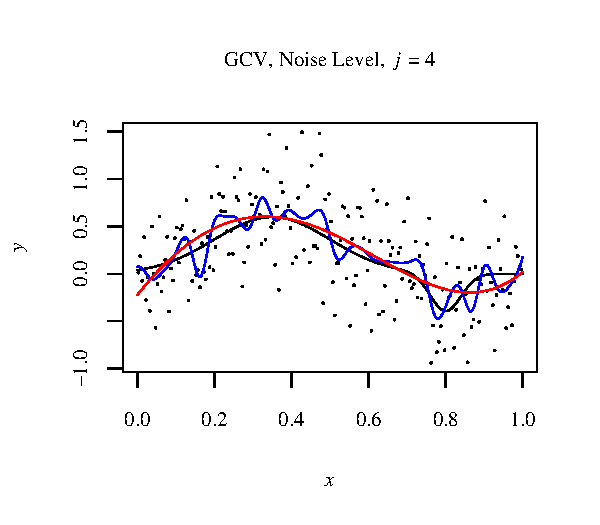
\includegraphics[width=1\linewidth,height=0.18\textheight]{Graphs/2/1/assignment5_a_2_1_4}&
      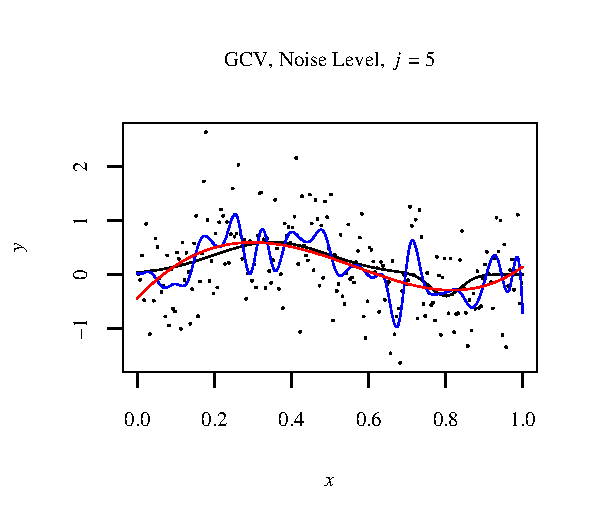
\includegraphics[width=1\linewidth,height=0.18\textheight]{Graphs/2/1/assignment5_a_2_1_5}&
      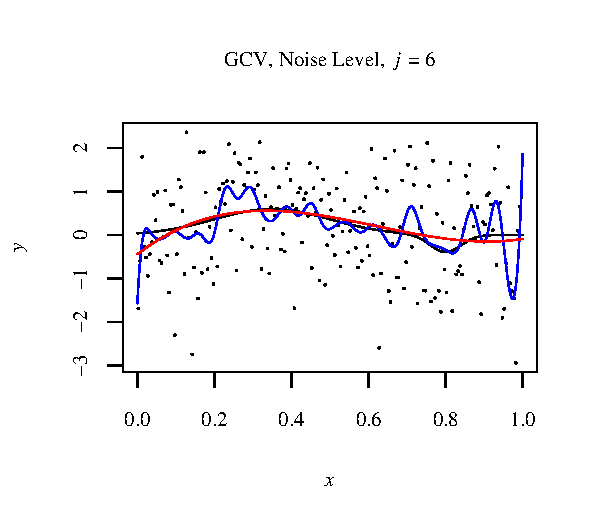
\includegraphics[width=1\linewidth,height=0.18\textheight]{Graphs/2/1/assignment5_a_2_1_6}\\\hline
    \end{tabular}
  \end{center}
\end{table*}

\begin{table*}[h!]
  \begin{center}
    \renewcommand{\arraystretch}{1.5}
    \begin{tabular}{| >{\centering\arraybackslash}m{2.1in} |  >{\centering\arraybackslash}m{2.1in} |  >{\centering\arraybackslash}m{2.1in}|}
      \hline
      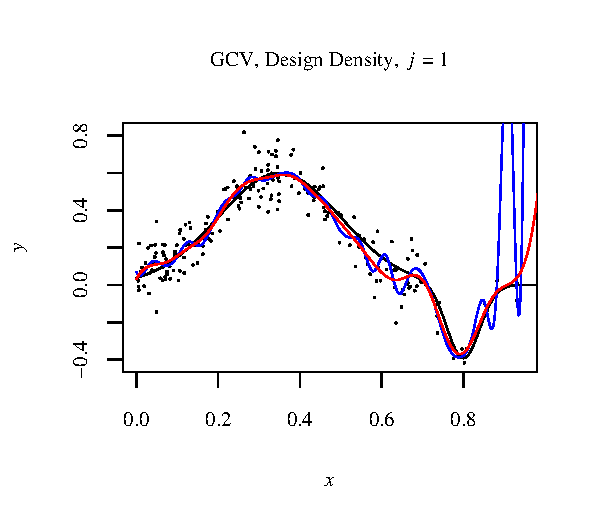
\includegraphics[width=1\linewidth,height=0.18\textheight]{Graphs/2/2/assignment5_a_2_2_1}&
      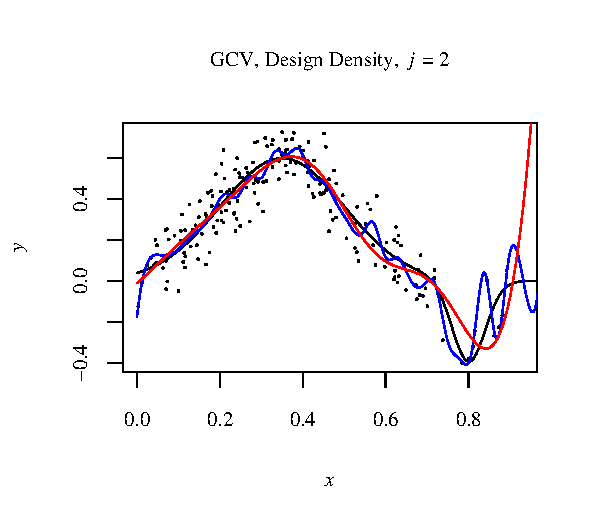
\includegraphics[width=1\linewidth,height=0.18\textheight]{Graphs/2/2/assignment5_a_2_2_2}&
      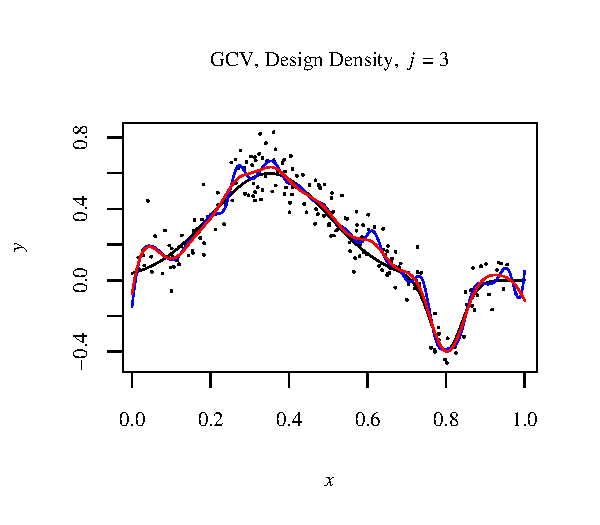
\includegraphics[width=1\linewidth,height=0.18\textheight]{Graphs/2/2/assignment5_a_2_2_3}\\\hline
      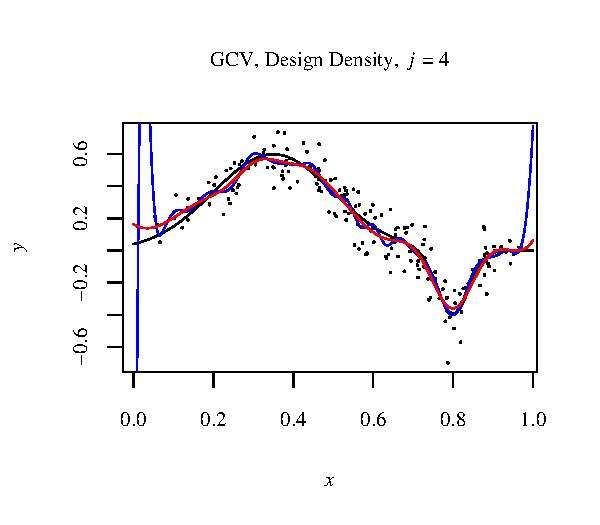
\includegraphics[width=1\linewidth,height=0.18\textheight]{Graphs/2/2/assignment5_a_2_2_4}&
      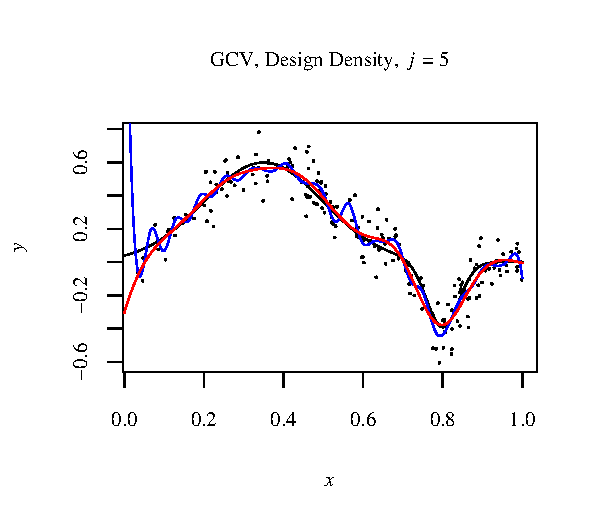
\includegraphics[width=1\linewidth,height=0.18\textheight]{Graphs/2/2/assignment5_a_2_2_5}&
      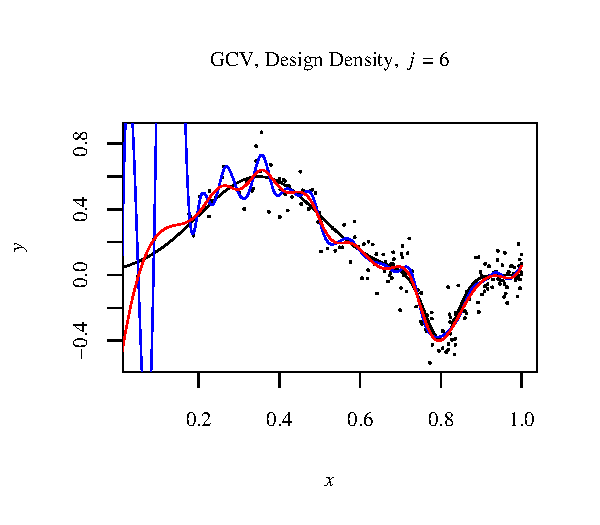
\includegraphics[width=1\linewidth,height=0.18\textheight]{Graphs/2/2/assignment5_a_2_2_6}\\\hline
    \end{tabular}
  \end{center}
\end{table*}

\begin{table*}[h!]
  \begin{center}
    \renewcommand{\arraystretch}{1.5}
    \begin{tabular}{| >{\centering\arraybackslash}m{2.1in} |  >{\centering\arraybackslash}m{2.1in} |  >{\centering\arraybackslash}m{2.1in}|}
      \hline
      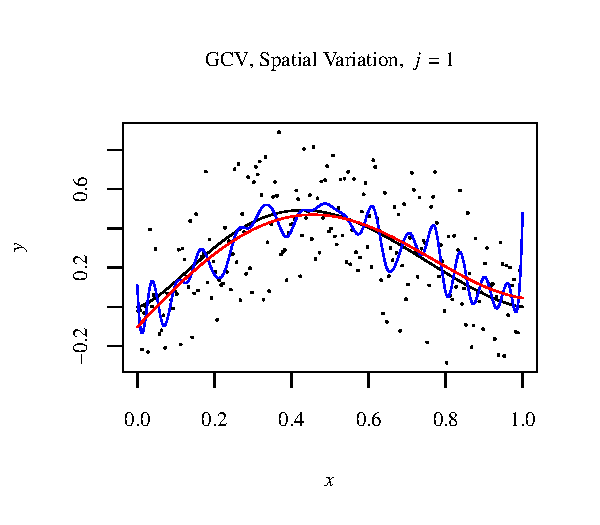
\includegraphics[width=1\linewidth,height=0.18\textheight]{Graphs/2/3/assignment5_a_2_3_1}&
      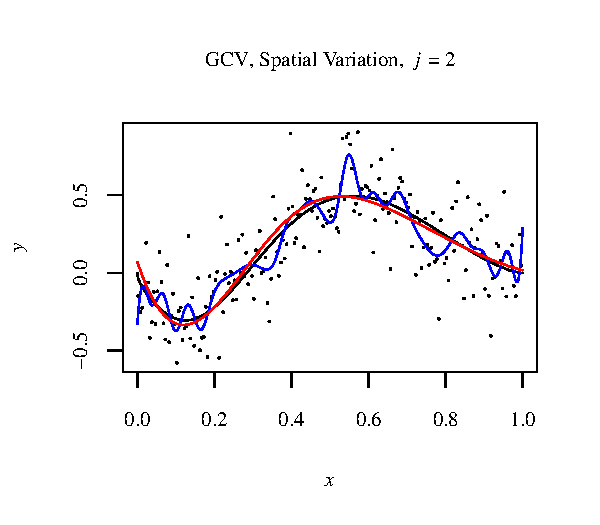
\includegraphics[width=1\linewidth,height=0.18\textheight]{Graphs/2/3/assignment5_a_2_3_2}&
      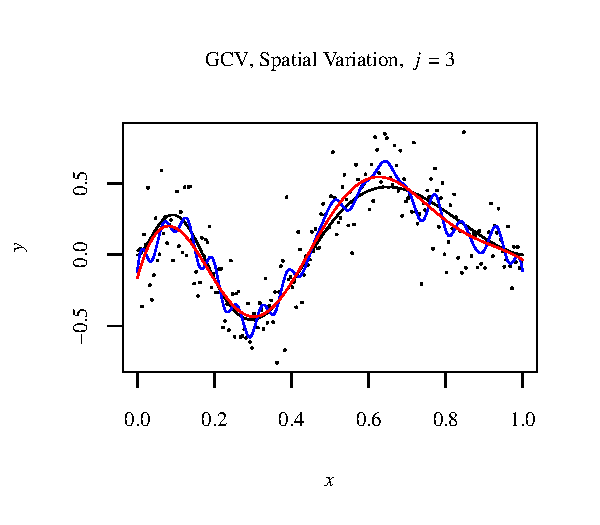
\includegraphics[width=1\linewidth,height=0.18\textheight]{Graphs/2/3/assignment5_a_2_3_3}\\\hline
      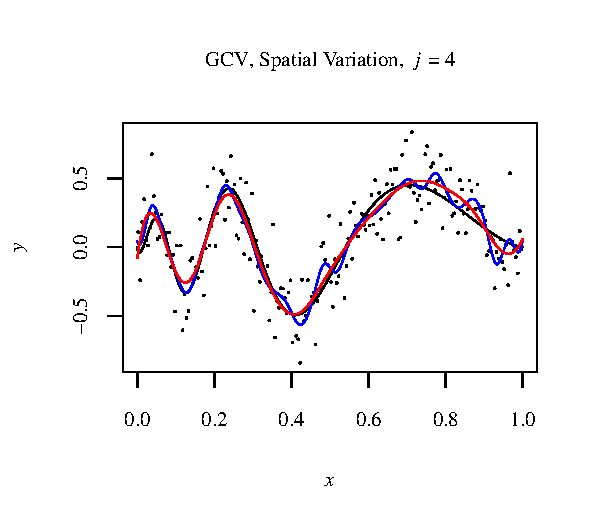
\includegraphics[width=1\linewidth,height=0.18\textheight]{Graphs/2/3/assignment5_a_2_3_4}&
      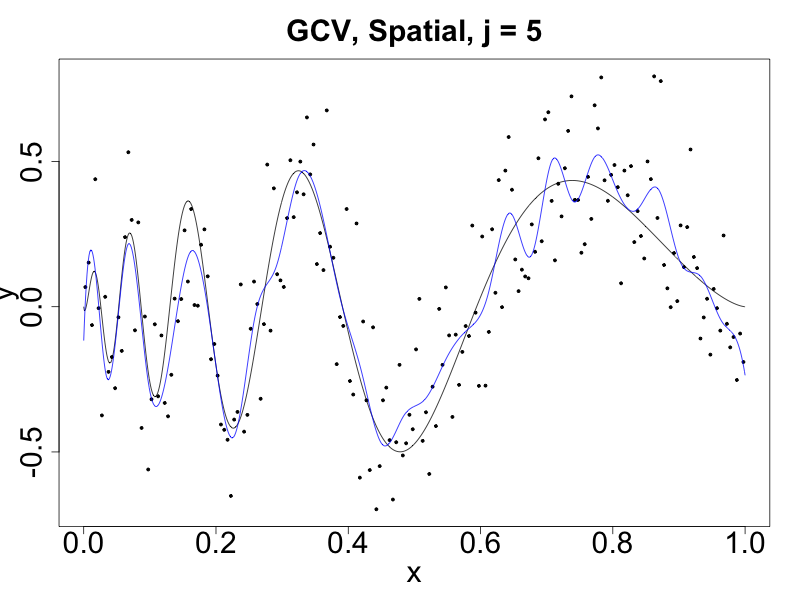
\includegraphics[width=1\linewidth,height=0.18\textheight]{Graphs/2/3/assignment5_a_2_3_5}&
      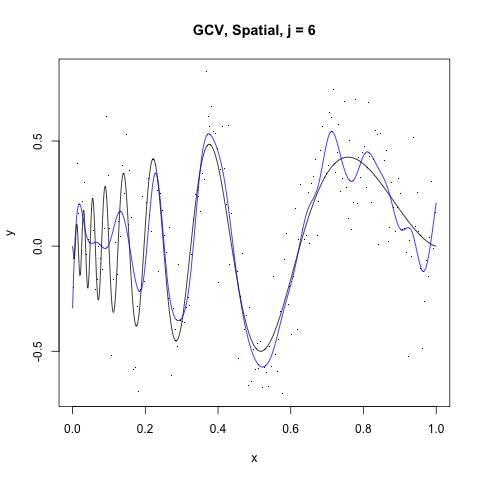
\includegraphics[width=1\linewidth,height=0.18\textheight]{Graphs/2/3/assignment5_a_2_3_6}\\\hline
    \end{tabular}
  \end{center}
\end{table*}

\begin{table*}[h!]
  \begin{center}
    \renewcommand{\arraystretch}{1.5}
    \begin{tabular}{| >{\centering\arraybackslash}m{2.1in} |  >{\centering\arraybackslash}m{2.1in} |  >{\centering\arraybackslash}m{2.1in}|}
      \hline
      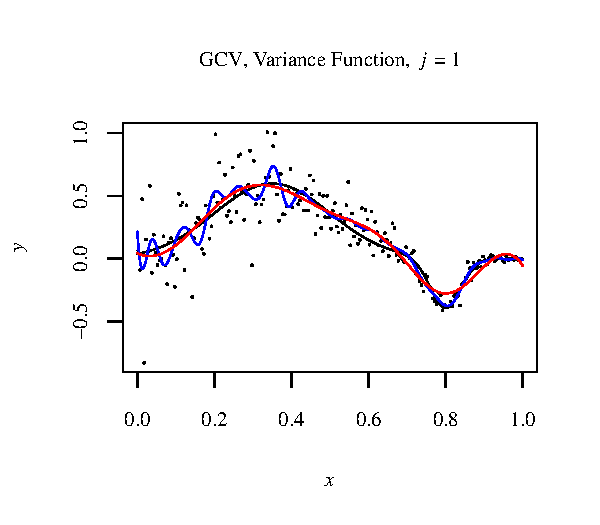
\includegraphics[width=1\linewidth,height=0.18\textheight]{Graphs/2/4/assignment5_a_2_4_1}&
      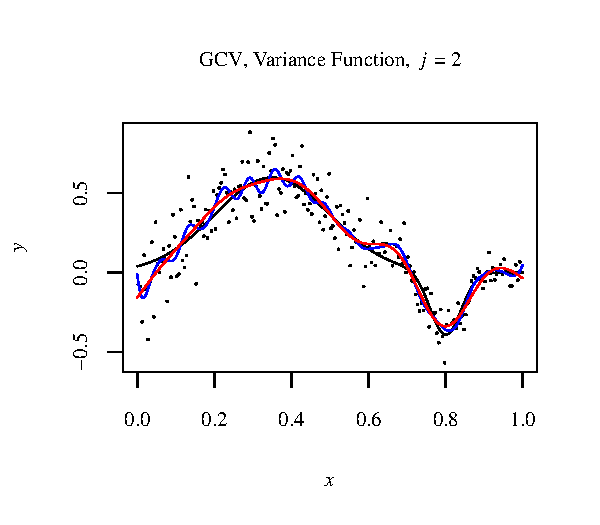
\includegraphics[width=1\linewidth,height=0.18\textheight]{Graphs/2/4/assignment5_a_2_4_2}&
      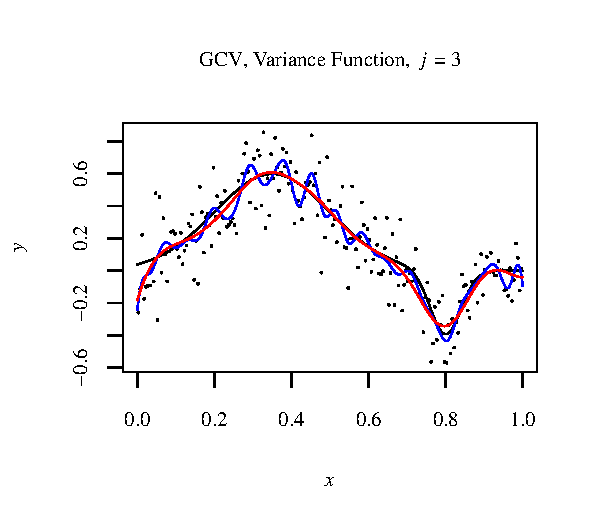
\includegraphics[width=1\linewidth,height=0.18\textheight]{Graphs/2/4/assignment5_a_2_4_3}\\\hline
      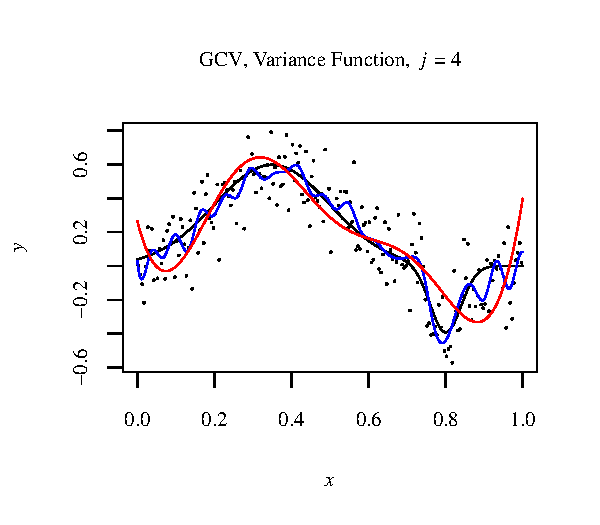
\includegraphics[width=1\linewidth,height=0.18\textheight]{Graphs/2/4/assignment5_a_2_4_4}&
      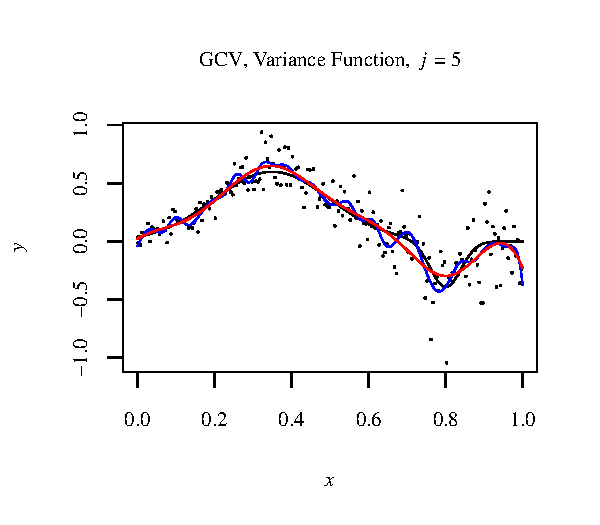
\includegraphics[width=1\linewidth,height=0.18\textheight]{Graphs/2/4/assignment5_a_2_4_5}&
      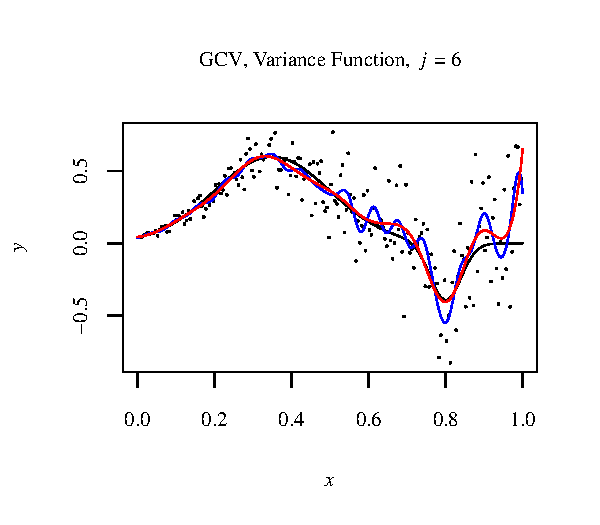
\includegraphics[width=1\linewidth,height=0.18\textheight]{Graphs/2/4/assignment5_a_2_4_6}\\\hline
    \end{tabular}
  \end{center}
\end{table*}

\begin{table*}[h!]
  \begin{center}
    \renewcommand{\arraystretch}{1.5}
    \begin{tabular}{| >{\centering\arraybackslash}m{2.1in} |  >{\centering\arraybackslash}m{2.1in} |  >{\centering\arraybackslash}m{2.1in}|}
      \hline
      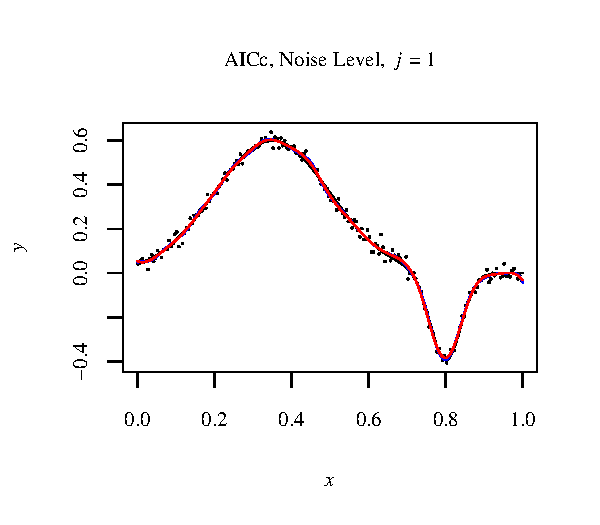
\includegraphics[width=1\linewidth,height=0.18\textheight]{Graphs/3/1/assignment5_a_3_1_1}&
      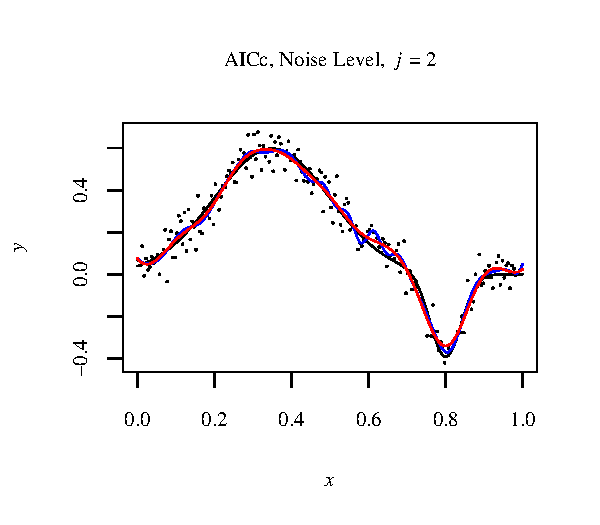
\includegraphics[width=1\linewidth,height=0.18\textheight]{Graphs/3/1/assignment5_a_3_1_2}&
      \includegraphics[width=1\linewidth,height=0.18\textheight]{Graphs/3/1/assignment5_a_3_1_3}\\\hline
      \includegraphics[width=1\linewidth,height=0.18\textheight]{Graphs/3/1/assignment5_a_3_1_4}&
      \includegraphics[width=1\linewidth,height=0.18\textheight]{Graphs/3/1/assignment5_a_3_1_5}&
      \includegraphics[width=1\linewidth,height=0.18\textheight]{Graphs/3/1/assignment5_a_3_1_6}\\\hline
    \end{tabular}
  \end{center}
\end{table*}

\begin{table*}[h!]
  \begin{center}
    \renewcommand{\arraystretch}{1.5}
    \begin{tabular}{| >{\centering\arraybackslash}m{2.1in} |  >{\centering\arraybackslash}m{2.1in} |  >{\centering\arraybackslash}m{2.1in}|}
      \hline
      \includegraphics[width=1\linewidth,height=0.18\textheight]{Graphs/3/2/assignment5_a_3_2_1}&
      \includegraphics[width=1\linewidth,height=0.18\textheight]{Graphs/3/2/assignment5_a_3_2_2}&
      \includegraphics[width=1\linewidth,height=0.18\textheight]{Graphs/3/2/assignment5_a_3_2_3}\\\hline
      \includegraphics[width=1\linewidth,height=0.18\textheight]{Graphs/3/2/assignment5_a_3_2_4}&
      \includegraphics[width=1\linewidth,height=0.18\textheight]{Graphs/3/2/assignment5_a_3_2_5}&
      \includegraphics[width=1\linewidth,height=0.18\textheight]{Graphs/3/2/assignment5_a_3_2_6}\\\hline
    \end{tabular}
  \end{center}
\end{table*}

\begin{table*}[h!]
  \begin{center}
    \renewcommand{\arraystretch}{1.5}
    \begin{tabular}{| >{\centering\arraybackslash}m{2.1in} |  >{\centering\arraybackslash}m{2.1in} |  >{\centering\arraybackslash}m{2.1in}|}
      \hline
      \includegraphics[width=1\linewidth,height=0.18\textheight]{Graphs/3/3/assignment5_a_3_3_1}&
      \includegraphics[width=1\linewidth,height=0.18\textheight]{Graphs/3/3/assignment5_a_3_3_2}&
      \includegraphics[width=1\linewidth,height=0.18\textheight]{Graphs/3/3/assignment5_a_3_3_3}\\\hline
      \includegraphics[width=1\linewidth,height=0.18\textheight]{Graphs/3/3/assignment5_a_3_3_4}&
      \includegraphics[width=1\linewidth,height=0.18\textheight]{Graphs/3/3/assignment5_a_3_3_5}&
      \includegraphics[width=1\linewidth,height=0.18\textheight]{Graphs/3/3/assignment5_a_3_3_6}\\\hline
    \end{tabular}
  \end{center}
\end{table*}

\begin{table*}[h!]
  \begin{center}
    \renewcommand{\arraystretch}{1.5}
    \begin{tabular}{| >{\centering\arraybackslash}m{2.1in} |  >{\centering\arraybackslash}m{2.1in} |  >{\centering\arraybackslash}m{2.1in}|}
      \hline
      \includegraphics[width=1\linewidth,height=0.18\textheight]{Graphs/3/4/assignment5_a_3_4_1}&
      \includegraphics[width=1\linewidth,height=0.18\textheight]{Graphs/3/4/assignment5_a_3_4_2}&
      \includegraphics[width=1\linewidth,height=0.18\textheight]{Graphs/3/4/assignment5_a_3_4_3}\\\hline
      \includegraphics[width=1\linewidth,height=0.18\textheight]{Graphs/3/4/assignment5_a_3_4_4}&
      \includegraphics[width=1\linewidth,height=0.18\textheight]{Graphs/3/4/assignment5_a_3_4_5}&
      \includegraphics[width=1\linewidth,height=0.18\textheight]{Graphs/3/4/assignment5_a_3_4_6}\\\hline
    \end{tabular}
  \end{center}
\end{table*}

\begin{table*}[h!]
  \begin{center}
    \renewcommand{\arraystretch}{1.5}
    \begin{tabular}{| >{\centering\arraybackslash}m{2.1in} |  >{\centering\arraybackslash}m{2.1in} |  >{\centering\arraybackslash}m{2.1in}|}
      \hline
      \includegraphics[width=1\linewidth,height=0.18\textheight]{Graphs/4/1/assignment5_a_4_1_1}&
      \includegraphics[width=1\linewidth,height=0.18\textheight]{Graphs/4/1/assignment5_a_4_1_2}&
      \includegraphics[width=1\linewidth,height=0.18\textheight]{Graphs/4/1/assignment5_a_4_1_3}\\\hline
      \includegraphics[width=1\linewidth,height=0.18\textheight]{Graphs/4/1/assignment5_a_4_1_4}&
      \includegraphics[width=1\linewidth,height=0.18\textheight]{Graphs/4/1/assignment5_a_4_1_5}&
      \includegraphics[width=1\linewidth,height=0.18\textheight]{Graphs/4/1/assignment5_a_4_1_6}\\\hline
    \end{tabular}
  \end{center}
\end{table*}

\begin{table*}[h!]
  \begin{center}
    \renewcommand{\arraystretch}{1.5}
    \begin{tabular}{| >{\centering\arraybackslash}m{2.1in} |  >{\centering\arraybackslash}m{2.1in} |  >{\centering\arraybackslash}m{2.1in}|}
      \hline
      \includegraphics[width=1\linewidth,height=0.18\textheight]{Graphs/4/2/assignment5_a_4_2_1}&
      \includegraphics[width=1\linewidth,height=0.18\textheight]{Graphs/4/2/assignment5_a_4_2_2}&
      \includegraphics[width=1\linewidth,height=0.18\textheight]{Graphs/4/2/assignment5_a_4_2_3}\\\hline
      \includegraphics[width=1\linewidth,height=0.18\textheight]{Graphs/4/2/assignment5_a_4_2_4}&
      \includegraphics[width=1\linewidth,height=0.18\textheight]{Graphs/4/2/assignment5_a_4_2_5}&
      \includegraphics[width=1\linewidth,height=0.18\textheight]{Graphs/4/2/assignment5_a_4_2_6}\\\hline
    \end{tabular}
  \end{center}
\end{table*}

\begin{table*}[h!]
  \begin{center}
    \renewcommand{\arraystretch}{1.5}
    \begin{tabular}{| >{\centering\arraybackslash}m{2.1in} |  >{\centering\arraybackslash}m{2.1in} |  >{\centering\arraybackslash}m{2.1in}|}
      \hline
      \includegraphics[width=1\linewidth,height=0.18\textheight]{Graphs/4/3/assignment5_a_4_3_1}&
      \includegraphics[width=1\linewidth,height=0.18\textheight]{Graphs/4/3/assignment5_a_4_3_2}&
      \includegraphics[width=1\linewidth,height=0.18\textheight]{Graphs/4/3/assignment5_a_4_3_3}\\\hline
      \includegraphics[width=1\linewidth,height=0.18\textheight]{Graphs/4/3/assignment5_a_4_3_4}&
      \includegraphics[width=1\linewidth,height=0.18\textheight]{Graphs/4/3/assignment5_a_4_3_5}&
      \includegraphics[width=1\linewidth,height=0.18\textheight]{Graphs/4/3/assignment5_a_4_3_6}\\\hline
    \end{tabular}
  \end{center}
\end{table*}

\begin{table*}[h!]
  \begin{center}
    \renewcommand{\arraystretch}{1.5}
    \begin{tabular}{| >{\centering\arraybackslash}m{2.1in} |  >{\centering\arraybackslash}m{2.1in} |  >{\centering\arraybackslash}m{2.1in}|}
      \hline
      \includegraphics[width=1\linewidth,height=0.18\textheight]{Graphs/4/4/assignment5_a_4_4_1}&
      \includegraphics[width=1\linewidth,height=0.18\textheight]{Graphs/4/4/assignment5_a_4_4_2}&
      \includegraphics[width=1\linewidth,height=0.18\textheight]{Graphs/4/4/assignment5_a_4_4_3}\\\hline
      \includegraphics[width=1\linewidth,height=0.18\textheight]{Graphs/4/4/assignment5_a_4_4_4}&
      \includegraphics[width=1\linewidth,height=0.18\textheight]{Graphs/4/4/assignment5_a_4_4_5}&
      \includegraphics[width=1\linewidth,height=0.18\textheight]{Graphs/4/4/assignment5_a_4_4_6}\\\hline
    \end{tabular}
  \end{center}
\end{table*}

\includepdf[pages={1-3}]{Code/assignment5.pdf}

\end{document}